\documentclass[aspectration=1610,t]{beamer}
\usepackage{csc}
\title{Лекция 6. Материалы и источники света}


\date{
   \textbf{ИТМО}\\
   19 октября 2022\\
   Санкт-Петербург
}

\begin{document}

\begin{frame}
  \titlepage
\end{frame}

\begin{frame}[fragile]{Представление цветов}
    \begin{itemize}
        \item {\bf RGB}
        \item {\bf HSV} - тон, насыщенность и яркость
        \item {\bf HSL} - тон, насыщенность и светлота
        \item и другие...
    \end{itemize}
\end{frame}

\begin{frame}[fragile]{Представление цветов HSL}
    \begin{figure}[htp]
        \centering
        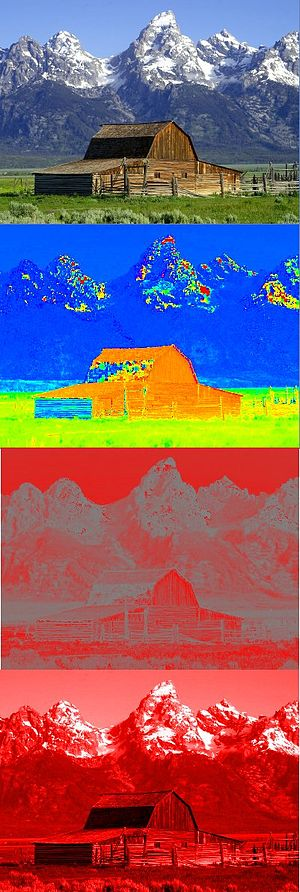
\includegraphics[scale=0.20]{res/hsl}
    \end{figure}
\end{frame}

\begin{frame}[fragile]{Смешивание цветов}
    {\bf multiply} - смешивает цвета, перемножая их. Получаемый цвет всегда будет темнее базового.
    \begin{figure}[htp]
        \centering
        
\includegraphics[scale=0.40]{res/multiply}
    \end{figure}
\end{frame}

\begin{frame}[fragile]{Смешивание цветов}
    {\bf multiply} - смешивает цвета, перемножая их. Получаемый цвет всегда будет темнее базового.
    \begin{figure}[htp]
        \centering
        
\includegraphics[scale=0.40]{res/multiply}
    \end{figure}
\end{frame}

\begin{frame}[fragile]{Смешивание цветов}
    {\bf hue} - смешивает цвета, изменяя оттенок базового цвета на оттенок смешиваемого, 
    сохраняя насыщенность и светлоту базового цвета.
    \begin{figure}[htp]
        \centering
        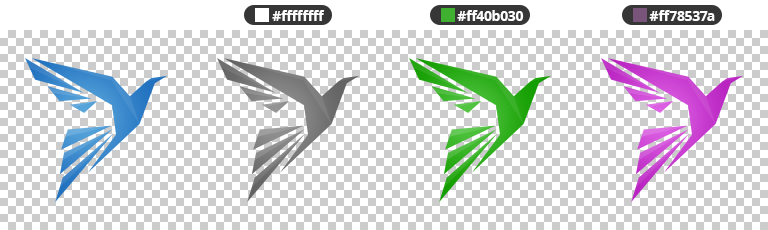
\includegraphics[scale=0.40]{res/hue}
    \end{figure}
\end{frame}

\begin{frame}[fragile]{Смешивание цветов}
    {\bf color} - cмешивает цвета, изменяя оттенок и насыщенность базового цвета на оттенок и 
    насыщенность смешиваемого, сохраняя светлоту базового цвета.
    \begin{figure}[htp]
        \centering
        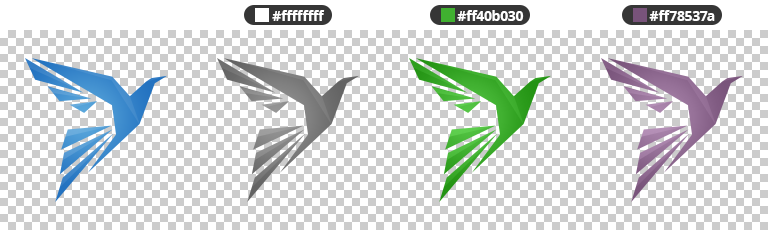
\includegraphics[scale=0.40]{res/color}
    \end{figure}
\end{frame}

\begin{frame}[fragile]{Смешивание цветов}
    {\bf difference} - смешивает цвета, вычитая меньшие значения из больших. 
    Смешение с белым цветом инвертирует цвет, с черным не дает изменений.
    \begin{figure}[htp]
        \centering
        
\includegraphics[scale=0.40]{res/difference}
    \end{figure}
\end{frame}

\begin{frame}[fragile]{Смешивание цветов}
    {\bf fill} - смешивает цвета, заливая непрозрачные пиксели базового цвета смешиваемым.
    Может использоваться для заливки прозрачных текстур с абстрактными формами.
    \begin{figure}[htp]
        \centering
        
\includegraphics[scale=0.40]{res/fill}
    \end{figure}
\end{frame}

\begin{frame}[fragile]{Материалы}
    Каждый объект по разному реагирует на свет.
    \begin{figure}[htp]
        \centering
        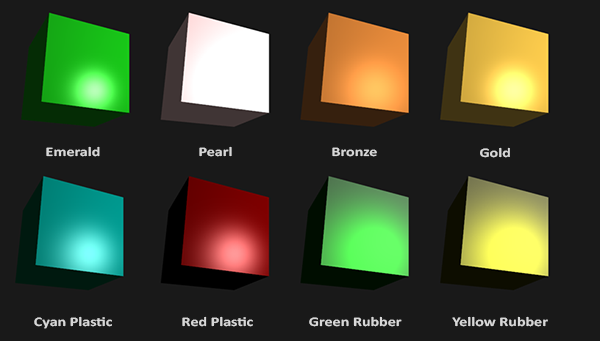
\includegraphics[scale=0.40]{res/materials}
    \end{figure}
\end{frame}

\begin{frame}[fragile]{Материалы}
    Удобно параметризовать конкретные объекты следующим образом.
    {\small \begin{lstlisting}
#version 330 core

struct Material {
    vec3 ambient;
    vec3 diffuse;
    vec3 specular;
    float shininess;
}; 
    
uniform Material material;
    \end{lstlisting}}
\end{frame}

\begin{frame}[fragile]{Компоненты материала}
    \begin{itemize}
        \item Вектор {\bf ambient} определяет, какой цвет объект отражает под фоновым освещением. Обычно это цвет самого объекта.
        \item Вектор {\bf diffuse} определяет цвет объекта под рассеянным освещением. Также, как и фоновый, он определяет желаемый цвет объекта.
        \item Вектор {\bf specular} устанавливает цвет блика на объекте, а переменная {\bf shininess} — радиус этого блика.
    \end{itemize}
\end{frame}

\begin{frame}[fragile]{Материалы}
    В коде шейдера необходимо учитывать материал:
    {\small \begin{lstlisting}
void main() {    
    // ambient
    vec3 ambient = lightColor * material.ambient;

    // diffuse 
    // ...
    vec3 diffuse = lightColor
        * (diff * material.diffuse);

    // specular
    // ...
    vec3 specular = lightColor
        * (spec * material.specular);  
}
    \end{lstlisting}}
\end{frame}

\begin{frame}[fragile]{Свойства источника света}
    Структура подобная материалу:
    {\small \begin{lstlisting}
#version 330 core

struct Light {
    vec3 position;

    vec3 ambient;
    vec3 diffuse;
    vec3 specular;
};

uniform Light light;
    \end{lstlisting}}
\end{frame}

\begin{frame}[fragile]{Свойства источника света}
    Параметризуем шейдер:
    {\small \begin{lstlisting}
vec3 ambient  = light.ambient * material.ambient;

vec3 diffuse  = light.diffuse 
    * (diff * material.diffuse);

vec3 specular = light.specular
    * (spec * material.specular); 
    \end{lstlisting}}
\end{frame}

\begin{frame}[fragile]{Текстурные карты}
    Только цвета не достаточно для представления более сложных объектов.
    Для представления таких объектов как правило используют текстурные карты.
    \begin{itemize}
        \item {\bf diffuse} - диффузная компонента, задает цвет;
        \item {\bf specular} - карта бликов, отражает силу бликов;
        \item {\bf normal} - карта нормалей (детали самой поверхности);
        \item И другие.
    \end{itemize}
\end{frame}

\begin{frame}[fragile]{Текстурные карты}
    В коде шейдера:
    {\small \begin{lstlisting}
#version 330 core

struct Material {
    sampler2D diffuse;
    sampler2D specular;
    sampler2D normal;
    float shininess;
}; 
    
uniform Material material;
    \end{lstlisting}}
\end{frame}

\begin{frame}[fragile]{Текстурные карты}
    Диффузная карта
    \begin{figure}[htp]
        \centering
        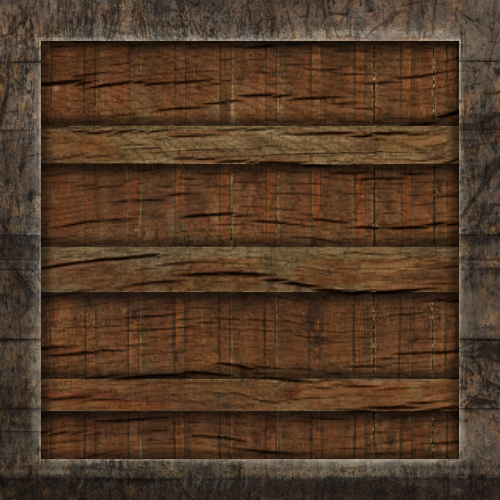
\includegraphics[scale=0.20]{res/diffuse_comp}
    \end{figure}
    Карта бликов
    \begin{figure}[htp]
        \centering
        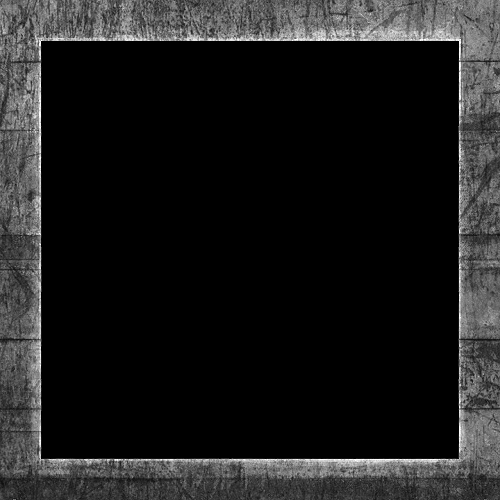
\includegraphics[scale=0.20]{res/specular_comp}
    \end{figure}
\end{frame}

\begin{frame}[fragile]{Текстурные карты}
    Их комбинация дает следующий результат
    \begin{figure}[htp]
        \centering
        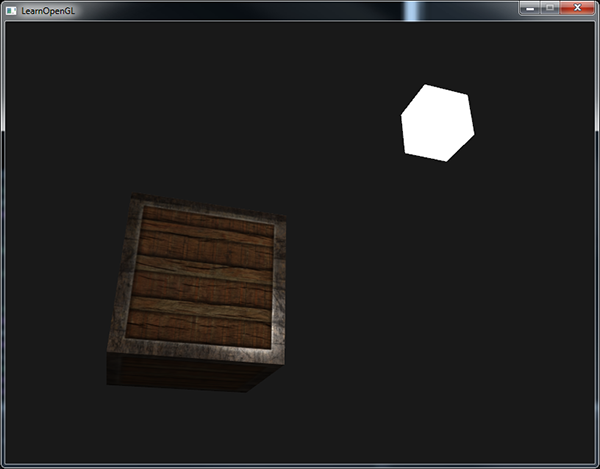
\includegraphics[scale=0.40]{res/diff_spec_combined}
    \end{figure}
\end{frame}

\begin{frame}[fragile]{Источники света}
    Основные типы источников:
    \begin{itemize}
        \item {\bf направленный} (directional)
        \item {\bf точечный} (point)
        \item {\bf прожектор} (spot)
    \end{itemize}
\end{frame}

\begin{frame}[fragile]{Направленный источник}
    \begin{figure}[htp]
        \centering
        
\includegraphics[scale=0.20]{res/directional}
    \end{figure}
    Параметризуется:
    {\small \begin{lstlisting}
struct Light {
    // no longer necessary when using directional lights.
    // vec3 position;
    vec3 direction;
    
    vec3 ambient;
    vec3 diffuse;
    vec3 specular;
};
    \end{lstlisting}}
\end{frame}

\begin{frame}[fragile]{Точечный источник}
    Светит во все стороны, однако интенсивность затухает.
    \begin{figure}[htp]
        \centering
        
\includegraphics[scale=0.2]{res/point}
    \end{figure}
    Как выбрать функцию для интенсивности?
    \begin{itemize}
        \item линейно
        \item квадратично
        \item иначе
    \end{itemize}
\end{frame}

\begin{frame}[fragile]{Точечный источник}
    Лучше всего себя показывает следующая зависимость интенсивности от расстояния $I(d) = \frac{1}{K_c + K_l \cdot d + K_q \cdot d^2}$
    \begin{figure}[htp]
        \centering
        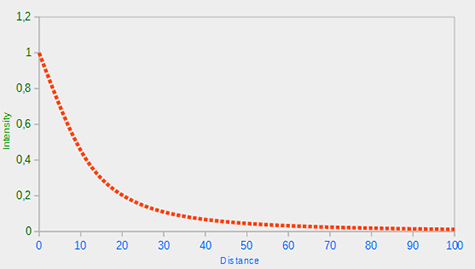
\includegraphics[scale=0.4]{res/attenuation.png}
    \end{figure}
\end{frame}

\begin{frame}[fragile]{Точечный источник}
    В шейдере же параметризуется:
    {\small \begin{lstlisting}
struct Light {
    vec3 position;  

    vec3 ambient;
    vec3 diffuse;
    vec3 specular;

    float constant;
    float linear;
    float quadratic;
}; 
    \end{lstlisting}}
\end{frame}

\begin{frame}[fragile]{Точечный источник}
    Для расчета затухания:
    {\small \begin{lstlisting}
float distance    = length(light.position - FragPos);
float attenuation = light.constant
    + light.linear * distance
    + light.quadratic * (distance * distance); 
    \end{lstlisting}}
    Применим к компонентам:
    {\small \begin{lstlisting}
ambient  *= 1. / attenuation; 
diffuse  *= 1. / attenuation;
specular *= 1. / attenuation;
    \end{lstlisting}}
\end{frame}

\begin{frame}[fragile]{Прожектор}
    Направленный пучок света. Ограниченный конусом
    \begin{figure}[htp]
        \centering
        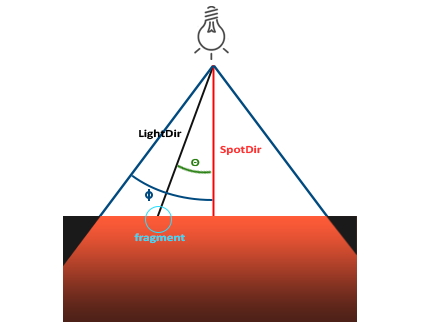
\includegraphics[scale=0.4]{res/spot}
    \end{figure}
\end{frame}

\begin{frame}[fragile]{Прожектор}
    В шейдере параметризуется:
    {\small \begin{lstlisting}
struct Light {
    vec3  position;
    vec3  direction;
    float cutOff;
    float outerCutOff;
    ...
};    
    \end{lstlisting}}
\end{frame}

\begin{frame}[fragile]{Прожектор}
    Для расчета света используем следущее соотношение:
    {\small \begin{lstlisting}
float theta = dot(lightDir, normalize(-light.direction));

if(theta > light.cutOff) { 
    // do lighting calculations
}
else {
    // else, use ambient light so scene 
    // isn't completely dark outside the spotlight.
}
    \end{lstlisting}}
\end{frame}

\begin{frame}[fragile]{Прожектор}
    Чтобы смягчить переход, необходимо задать затухание между внутренним и внешним конусами
    $I(\theta) = \frac{\theta - \gamma}{\epsilon}, \epsilon = \phi - \gamma$
    \begin{itemize}
        \item $\gamma$ - внешний угол
        \item $\phi$ - внутренний
        \item $\epsilon$ - разница углов
    \end{itemize}
    {\small \begin{lstlisting}
float theta = dot(lightDir,
    normalize(-light.direction));
float epsilon = light.cutOff - light.outerCutOff;
float intensity = clamp(
    (theta - light.outerCutOff) / epsilon, 0.0, 1.0);

...

diffuse  *= intensity;
specular *= intensity;
    \end{lstlisting}}
\end{frame}

\end{document}

